
\documentclass[journal]{IEEEtran}
\usepackage{cite} 
\usepackage{graphicx} 
% NOTE: for dual use with latex and pdflatex, instead load graphicx like:
%\ifx\pdfoutput\undefined
%\usepackage{graphicx}
%\else
%\usepackage[pdftex]{graphicx}
%\fi
\usepackage{psfrag}
\usepackage{subfigure} 
\usepackage{url}
\usepackage{stfloats} 
\usepackage{amsmath}  
\interdisplaylinepenalty=2500
\usepackage{array}
\makeatletter
 \let\NAT@parse\undefined
 \makeatother
\ifx\pdfoutput\undefined
\usepackage[hypertex]{hyperref}
\else
\usepackage[pdftex,hypertexnames=false]{hyperref}
\fi
\usepackage[utf8]{inputenc}
\usepackage{amssymb, amsmath, amsbsy} % simbolitos
\usepackage{upgreek} % para poner letras griegas sin cursiva
\usepackage{cancel} % para tachar
\usepackage{mathdots} % para el comando \iddots
\usepackage{mathrsfs} % para formato de letra
\usepackage{stackrel} % para el comando \stackbin

\hyphenation{op-tical net-works semi-conduc-tor}


\begin{document}
%
% paper title
\title{Modelo no ideal del capacitor: Modelo de perdidas electromagnéticas para carga en tensión directa de un condensador}
%
%
% author names and IEEE memberships
% note positions of commas and nonbreaking spaces ( ~ ) LaTeX will not break
% a structure at a ~ so this keeps an author's name from being broken across
% two lines.
% use \thanks{} to gain access to the first footnote area
% a separate \thanks must be used for each paragraph as LaTeX2e's \thanks
% was not built to handle multiple paragraphs
\author{Keylor~Mena,\\~\IEEEmembership{Estudiante,~Instituto Tecnológico de Costa Rica,\\~SESLab,}
        % <-this % stops a space
\thanks{Manuscript received January 20, 2002; revised November 18, 2002.}% <-this % stops a space
\thanks{K. Mena esta con el Tecnologico de Costa Rica.}}
% note the % following the last \IEEEmembership and also the first \thanks - 
% these prevent an unwanted space from occurring between the last author name
% and the end of the author line. i.e., if you had this:
% 
% \author{....lastname \thanks{...} \thanks{...} }
%                     ^------------^------------^----Do not want these spaces!
%
% a space would be appended to the last name and could cause every name on that
% line to be shifted left slightly. This is one of those "LaTeX things". For
% instance, "A\textbf{} \textbf{}B" will typeset as "A B" not "AB". If you want
% "AB" then you have to do: "A\textbf{}\textbf{}B"
% \thanks is no different in this regard, so shield the last } of each \thanks
% that ends a line with a % and do not let a space in before the next \thanks.
% Spaces after \IEEEmembership other than the last one are OK (and needed) as
% you are supposed to have spaces between the names. For what it is worth,
% this is a minor point as most people would not even notice if the said evil
% space somehow managed to creep in.
%
% The paper headers
\markboth{Journal of \LaTeX\ Class Files,~Vol.~1, No.~11,~November~2002}{Shell \MakeLowercase{\textit{et al.}}: Bare Demo of IEEEtran.cls for Journals}
% The only time the second header will appear is for the odd numbered pages
% after the title page when using the twoside option.
% 
% *** Note that you probably will NOT want to include the author's name in ***
% *** the headers of peer review papers.                                   ***

% If you want to put a publisher's ID mark on the page
% (can leave text blank if you just want to see how the
% text height on the first page will be reduced by IEEE)
%\pubid{0000--0000/00\$00.00~\copyright~2002 IEEE}

% use only for invited papers
%\specialpapernotice{(Invited Paper)}

% make the title area
\maketitle


\begin{abstract}

When designing energy storage systems the analysis of parasitic components within the system is important, they provide an idea of how much of the energy supplied in this system is exploited. \\
Typically, systems use capacitors or supercapacitors as storage devices, because they can store voltage easily. Although in many systems these are considered as ideal components, the parasitic components of these have a noticeable effect on their functioning.\\
In order to take into account these parasitic effects, non-ideal models are used; In these models the ideal component is accompanied by other components that represent the effects of the parasitic loads. \\ There are different models that help to represent more precisely specific effects of the components, in this report we will look for a model that will help us to represent more Accuracy of the charging process of a capacitor.
\end{abstract}

\begin{keywords}
Capacitores, efectos parásitos, sistemas de almacenamiento, modelos no ideales.
\end{keywords}
% Note that keywords are not normally used for peerreview papers.

% For peer review papers, you can put extra information on the cover
% page as needed:
% \begin{center} \bfseries EDICS Category: 3-BBND \end{center}
%
% For peerreview papers, inserts a page break and creates the second title.
% Will be ignored for other modes.
\IEEEpeerreviewmaketitle



\section{Introducción}
% The very first letter is a 2 line initial drop letter followed
% by the rest of the first word in caps.
% 
% form to use if the first word consists of a single letter:
% \PARstart{A}{demo} file is ....
% 
% form to use if you need the single drop letter followed by
% normal text (unknown if ever used by IEEE):
% \PARstart{A}{}demo file is ....
% 
% Some journals put the first two words in caps:
% \PARstart{T}{his demo} file is ....
% 
% Here we have the typical use of a "T" for an initial drop letter
% and "HIS" in caps to complete the first word.
\PARstart{A}{l} diseñar sistemas de almacenamiento de energía el análisis de componentes parásitos dentro del sistema es importante, estas proporcionan una idea de cuanta de la energía suministrada en este es aprovechada. \\
Usualmente los sistemas usan como dispositivos de almacenamiento capacitores o supercapacitores, ya que estos permiten almacenar voltaje fácilmente. Aunque en muchos sistemas estos se consideran como componentes ideales, los componentes parásitos de estos tienen efectos notorios en su funcionamiento.\\ Para poder tomar en cuenta estos efectos parásitos, se utilizan modelos no ideales; en estos modelos el componente ideal es acompañado por otros componentes que representan los efectos de las cargas parásitas.\\ Existen distintos modelos que ayudan a representar mas precisamente efectos específicos de los componentes, en este informe buscaremos un modelo que nos ayude a representar con mas exactitud el proceso de carga de un capacitor. 


\subsection{Datos básicos del capacitor}
"La capacitancia C del capacitor es la razón de la magnitud de la carga en una de las placas a la diferencia de magnitud entre ellas. De esta manera podemos describir la capacitancia como en la formula \ref{eq:Ecu_cap}.

\begin{equation}
\label{eq:Ecu_cap}
C=\frac{Q}{V}=\frac{\varepsilon \oint Eds}{\int Edl}
\end{equation}
"\cite{Hayt}
\\Si despejamos la carga en términos de la capacitancia y el voltaje en la ecuación \ref{eq:Ecu_cap}, podemos afirmar que: capacitancia es una medida de la capacidad de almacenar energía en forma de carga separada o de una campo eléctrico.\\ En general la carga almacenada varia en función del tiempo, por lo que podemos escribir la corriente en el capacitor como en la ecuación \ref{eq:Ecu_Icap}.

\begin{equation}
\label{eq:Ecu_Icap}
i(t)=\frac{\partial }{\partial t}q(t)=C\frac{\partial }{\partial t}v(t)
\end{equation}

Despejando el voltaje de la ecuación \ref{eq:Ecu_Icap} se puede definir escribir la tensión del capacitor como en la ecuación \ref{eq:Ecu_Vcap}.

\begin{equation}
\label{eq:Ecu_Vcap}
V(t)=\frac{1}{C}\oint_{-\infty }^{t}i(\tau )d\tau 
\end{equation}

En la ecuación \ref{eq:Ecu_Vcap} podemos ver que el voltaje en un capacitor no puede cambiar instantáneamente.\cite{dorf} \\Definiendo la impedancia del capacitor como la ley de ohm usaremos la ecuación de la corriente del capacitor para definir la corriente de la ecuación \ref{eq:Ecu_Icap} en términos del voltaje del capacitor, pero para eliminar el diferencial transformaremos la corriente al dominio de la frecuencia usando la transformada de fourier, definiendo la impedancia como la ecuación \ref{eq:Ecu_Zcap}.
\[\frac{\partial X(t))}{\partial t}=j\omega X(j\omega )\] \cite{modelos}
\begin{equation}
\label{eq:Ecu_Zcap} 
Z(j\omega )=\frac{V(j\omega )}{j\omega V(j\omega )}=\frac{1}{j\omega }
\end{equation} 
La impedancia de la ecuación \ref{eq:Ecu_Zcap} dice que en una corriente de cero la impedancia del capacitor es infinita, la cual se vería como un abierto. Mientras a frecuencias que tiendan a infinito la resistencia sera de cero viéndose como un cable.\\ Con estos conceptos claros podemos comenzar a analizar el modelo ideal del capacitor.
% needed in second column of first page if using \pubid
%\pubidadjcol
 
\subsubsection{Modelo ideal del capacitor}
La fórmula \ref{eq:Ecu_Zcap} describe cómo se ve la impedancia de un capacitor en el dominio de la frecuencia, donde mientras más alta sea la frecuencia más pequeña es la impedancia que presenta el capacitor.\\
Esto puede causar que la impedancia del capacitor pueda variar entre un corto o un abierto, una resistencia de cero en frecuencia que tiendan a infinito o impedancias infinitas en corriente directa.\\ Este efecto se puede notar en la ecuación \ref{eq:Ecu_Zcap}, donde se aprecia la relación de la impedancia capacitiva en términos del dominio de la frecuencia.\\Esto implica que al estar expuestos una un voltaje invariante en el tiempo, la corriente a través del capacitor es cero,y por lo tanto, como dicta ecuación \ref{eq:Ecu_Icap}, si no hay corriente el cambio de tensión en el capacitor es cero\\ Esto causa que en un capacitor ideal, la tensión entre sus terminales no pueda disminuir sino se se le aplica una tensión mas baja o por defecto se cortocircuiten sus terminales, por lo tanto una capacitor ideal mantiene su tensión ilimitadamente al estar al aire.


\subsection{Modelo no ideal del capacitor}
Con mencionamos antes, un capacitor ideal suele ser un dispositivo que almacena toda la carga que se le suministra, ademas su resistencia puede llegar a ser infinita o cero, dependiendo de la frecuencia con la que se exponga. \\ No obstante estos efectos no se cumplen en la vida real. Para remediar este efecto, vamos a realizar 2 modificaciones fundamentales al modelo del capacitor; la resistencia de dieléctrico y las perdidas RL en serie. 

\subsubsection{Resistencia del dieléctrico}
 La construcción de los capacitores requiere de un material no conductor que separe la placa y de esta manera poder almacenar el campo eléctrico; no obstante, aunque estos elementos posean impedancias muy altas nunca llegan a ser infinitas.\\ Este efecto puede ser modelado con una resistencia en paralelo al capacitor representando la resistencia del dieléctrico o el material no conductor que separa las placas.\\ Este efecto resistivo del dieléctrico genera las siguientes consecuencias:
 \begin{itemize}
 	\item \textbf{Corriente de fuga a través del dieléctrico:} debido a que la resistencia presente en el dieléctrico no puede llegar a ser infinita, por esta siempre va a circular una corriente.
 	 \item \textbf{Auto descarga del capacitor: } debido a que la corriente que atraviesa al capacitor nuca llega a ser cero siempre va a existir un cambio de voltaje,basados en la ecuación \ref{eq:Ecu_Icap}. Por lo que un capacitor que se encuentre con sus terminales al aire comenzara a perder su tensión almacenada sin ningún estimulo externo.
 	 \item \textbf{Reducción de la tensión almacenada: } Con el modelo ideal el capacitor podía tener una resistencia infinita, en donde todo el voltaje de fuente al final se almacenaría en el capacitor. Ya que esta resistencia no puede ser infinita, se debe aplicar un divisor de tensión. No obstante ya que la resistencia del dieléctrico ronda por los 10 M\(\Omega\) la tensión que cae en el capacitor sera muy semejante a la de la fuente
 	  
 \end{itemize}
 
 \subsubsection{Carga en serie del capacitor: }Para determinar el valor de la capacitancia, se usa la formula \ref{eq:Ecu_cap}, sin embargo, para determinar la capacitancia depende mas de los parámetros de construcción (área de las placas, la separación entre estas y el dieléctrico).\\ En el modelo ideal calculo se utilizan se ignorando valores de las resistencias de los contactos y la inductancia que se genera en el capacitor. Estos componentes se generan debido a que, de manera equivalente al capacitor, estos parámetros de la inductancia dependen de los parámetros de construcción de este \cite{Saiku}.\\En el caso de la resistencia, la formula para calcular se muestra en la ecuación \ref{eq:Resistencia}: 
 
 \begin{equation}
 \label{eq:Resistencia}
 R=\frac{V}{I}=\frac{\int Edl}{\sigma \oint Eds}
 \end{equation}
 
 Mientras que la inductancia se muestra en la ecuación \ref{eq:inductancia} 
 
 \begin{equation}
 \label{eq:inductancia}
 L=\frac{\Phi }{I}=\frac{\mu \int ds}{ \oint dl}
 \end{equation}
 
 Debido a esto siempre va a existir una resistencia y una inductancia en serie al capacitor, simulando las perdidas de estos elementos intrínsecos del capacitor.\\ Para modelar estos componentes existen 2 maneras, poner la resistencia y el inductor en paralelo o en serie, tal y como se muestra en la figura \ref{fig:circuitos_equivalentes}.\\ Generalmente se usa el modelo donde el inductor y la resistencia están en serie. Pero para simular la carga en un capacitor este modelo genera algunos problemas.
 \begin{itemize}
 	\item Las resistencias parásitas en serie cierran el circuito causando que una corriente existe a estas y comiencen con un voltaje inicial, esto implica que no se pueda simular la carga del capacitor desde cero. 
	\item Si se introduce un escalo unitario el inductor detectara un cambio muy rápido en el voltaje, elevando su impedancia, haciendo que la resistencia de entrada del capacitor en un inicio parezca un abierto al inicio y todo el voltaje caiga en este al inicio.
 	\item El inductor en parásito aumenta su impedancia conforme la frecuencia incrementa, dificultando que el capacitor actué con un corto en frecuencia muy altas.
 \end{itemize}
 
 \begin{figure}[hbtp]
 	\centering
 	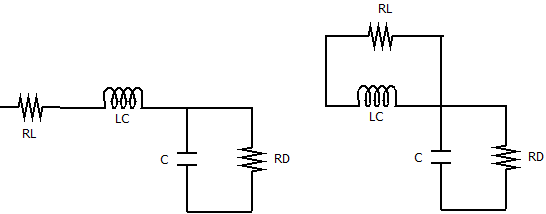
\includegraphics[width=2.5in]{img/Circutos_equivalentes.png}
 	\caption{Circuitos equivalentes del capacitor, con el circuito RL en paralelo y serie}
 	\label{fig:circuitos_equivalentes}
 \end{figure} 
 Si se parametrizan estos componentes en intervalos de la frecuencia específicos este modelo alcanza valores muy parecido a los de la realidad. Sin embargo, para estos experimentos usaremos la resistencia y el inductor en paralelo.\\ En este modelo el inductor minimiza el efecto de la resistencia en bajas frecuencias cortocircuitando esta y convirtiéndolo en un corto, mientras que la resistencia limita el valor máximo de impedancia que puede alcanzar el inductor en altas frecuencias, ya que al estar en paralelo, el valor máximo que se puede alcanzar es el de esta resistencia cuando el inductor alcanza impedancias cercanas a infinito. El inductor limita l tiempo en el que la resistencia del inductor ejerce efecto en el circuito\\
 Para analizar los efectos de este inductor en el circuito se usara la segunda ley de Maxwell \cite{Saiku}, se puede notar en la ecuación \ref{eq:segunda_ley_de_maxwell}.\\
 Esta ecuación dicta una generalización de la ley de voltajes de Kirchhoff, donde la sumatoria de todas las tensiones o cargas en un circuito cerrado debe sumar cero, pero a diferencia de la ley de Kirchhoff, la ecuación \ref{eq:segunda_ley_de_maxwell} dice que si existe una diferencia de tensión en una trayectoria cerrada esta se vera como un cambio en el campo magnético a través del tiempo.\\
 
  \begin{equation}
  \label{eq:segunda_ley_de_maxwell}
  \bigtriangledown \times E=\oint Edl=-\frac{\partial B}{\partial t}
  \end{equation}
  
  Este efecto se vera en el inductor parásito, donde este disminuye o crea un diferencial de tensión en el circuito disminuyendo la tensión del capacitor, sin embargo como se menciono antes, este efecto solo sera apreciable durante un tiempo definido por el valor del inductor.\\ Este efecto no se considera usualmente en la formula de la carga del capacitor.
  
 \subsection{Metodología}
 Para determinar los elementos parásitos del capacitor se ocupara:
 \begin{itemize}
 	\item Una fuente de voltaje directo, en este experimento se usara la fuente B2900 de Agilent, aprovechando que esta proporciona una gran precisión de voltaje y corriente.
 	\item Osciloscopio
 	\item Generador de funciones
 \end{itemize}
 Para minimizar el factor de error en los elementos parásitos se calcularan primero los elementos parásitos de los componentes de medición y las fuentes usadas.\\ 
 Para determinar los valores de las cargas parásitas, se usaran los circuitos de las figuras \ref{fig:Medicion_Ro} y \ref{fig:Medicion_Rf}. En estos se presenta una resistencia 'Rp' esta es la resistencia de carga del capacitor, su valor es determinado por medio de la fuente de voltaje usado, ya que la fuente usada puede medir resistencias con una gran precisión.  
 
 \begin{figure}
 \centering
 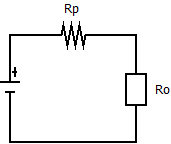
\includegraphics[width=2in]{img/Medicion_Ro}
 \caption{circuito de Medición de la resistencia del Osciloscopio}
 \label{fig:Medicion_Ro}
 \end{figure}
 
  \begin{figure}
  	\centering
  	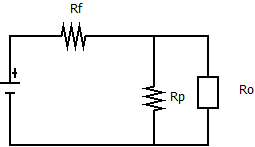
\includegraphics[width=2.5in]{img/Medicion_Rf}
  	\caption{circuito de Medición de la resistencia de la fuente}
  	\label{fig:Medicion_Rf}
  \end{figure}
  
  Con estos valores se podrán determinar son mayor precisión los valores parásitos del capacitor usando solo el circuito de medición de la figura \ref{fig:Medicion_de_medicion}. En esta se etiqueta la resistencia de fuente como Rd, la resistencia en paralelo del inductor como Rl y el inductor como Lc.
  
  \begin{figure}
  	\centering
  	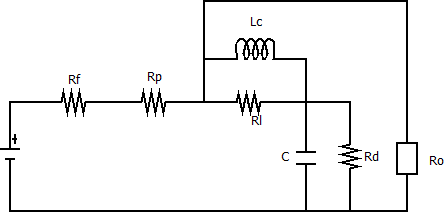
\includegraphics[width=2.5in]{img/Circuito_de_medicion}
  	\caption{circuito de Medición para los elementos parásitos del circuito}
  	\label{fig:Medicion_de_medicion}
  \end{figure}
  
  Usando esto determinaremos el valor de la resistencia del dieléctrico usando la formula de Ohm, midiendo el voltaje que da el Osciloscopio a la salida cuando no hay cambio en el voltaje, en este momento el inductor eliminaría los efectos de la resistencia Rl y el capacitador actuaria como un abierto; por lo que al dividir este valor de voltaje entre la corriente brinda por la fuente tendríamos el valor del voltaje de salida, sin embargo como se muestra en la figura \ref{fig:Medicion_de_medicion}, esta resistencia quedaría en paralelo a la resistencia del osciloscopio, por lo que, la ecuación que da el valor de la resistencia del dieléctrico se describe en la ecuación \ref{eq:resitencia_del_dielectrico}.
  
  \[R_{salida}=\frac{V_{medido}}{I_{fuente}}\]
  \begin{equation}
  \label{eq:resitencia_del_dielectrico}
  R_{dielectico}=\frac{R_{salida}*R_{osciloscopio}}{R_{osciloscopio}-R_{salida}}
  \end{equation}
  
  Para determinar la resistencia 'Rl', usaremos una aproximación parecida a la usada para determinar la resistencia del dieléctrico. En este caso usaremos un generador de funciones y alimentaremos el circuito con la mayor frecuencia posible.\\Debido a esto, el capacitor reducirá el efecto de la resistencia del dieléctrico y el inductor actuara como un abierto, por lo tanto la única resistencia de salida sera la del inductor.\\ En este caso asumiremos que la corriente del circuito se dividirá en 2, la que pasa por la resistencia y la que pasa por el osciloscopio, en este caso la ecuación que describe la resistencia de la bobina esta en la formula \ref{eq:resitencia_del_inductor}.
  \begin{equation}
  \label{eq:resitencia_del_inductor}
  R_{L}=\frac{V_{medido}}{I}
  \end{equation}
  Donde la corriente se define como:\\
  \[I=\overbrace{\frac{V_{fuente}-V_{medido}}{R_{fuente}+R_{carga}}}^{corriente total}-\underbrace{\frac{V_{medido}}{R_{osciloscopio}}}_{corriente osciloscopio}\]
  En este caso la resistencia de fuente debe calcularse igual de la fuente de corriente directa, pero es recomendable trabajar a la misma frecuencia y tensión que en la prueba, ya que algunos generados varían su potencia entregada dependiendo de la frecuencia.\\ 
  Para analizar fácilmente el circuito y determinar la inductancia parásita, determinaremos la función de transferencia de la circuito de la figura \ref{fig:Medicion_de_medicion} como en la ecuación \ref{eq:funcion_de_transferencia} 
  \begin{equation}
  \label{eq:funcion_de_transferencia}
  V_{cap}=\frac{V_{f}}{S}\frac{ALS^{2}+BLS+C}{DS^{2}+ES+FLS+G}
  \end{equation}
  Donde:\\
  \[A=R_{L}R_DC\]
  \[B=(R_D+R_L)\]
  \[C=R_LR_D\]
  \[D=(R_P+R_L)R_DC\]
  \[E=R_LR_DC\]
  \[F=(R_P+R_D+R_l)\]
  \[G=R_PR_L+R_LR_D\]
  Si tomamos el voltaje del capacitor como una porción de la tensión de la fuente establecida por el tiempo que el capacitor se carga, podemos escribir el voltaje del capacitor como \(V_{cap}=\tau V\), despejando L podemos establece una ecuación \ref{eq:indutor_funcion}. 
  \begin{equation}
  \label{eq:indutor_funcion}
  L=k*\frac{S^{3}+\alpha S^{2}+\beta S+\epsilon }{S(1+\delta S)}
  \end{equation}
  donde:
  \[\alpha=R_{L}\]
  \[\beta=\frac{R_L}{R_DC}\]
  \[\epsilon=\frac{R_L}{(R_P+1)C\tau}\]
  \[\delta=\frac{R_D+R_L}{R_DR_LC-\tau (R_p+1)}\]
  \[k=\frac{R_DR_LC-\tau (R_p+1)}{(R_P+1)R_DC\tau}\]
  La ecuación \ref{eq:indutor_funcion} es una ecuación impropia,  por lo cual no podemos pasarla al dominio del tiempo directamente. Por lo tanto en este caso usaremos diagramas de Bode para representar el valor del inductor de manera gráfica, como estamos trabajando con la carga en tensión directa de un capacitor, buscaremos el valor en la gráfica de frecuencia 0.
  Si partimos de la ecuación \ref{eq:funcion_de_transferencia} para definir una ecuación de diferencias de entrada salida podemos definir la ecuación \ref{eq:diferencias_ES}, donde se nota que los cambios en el voltaje del capacitor quedan dependiendo de la entrada y de sus derivadas de la entrada, como la entrada se define como un escalón unitario en cero, las derivadas al inicio tenderán a ser muy alta.
  \begin{equation}
  \label{eq:diferencias_ES}
 DV_{cap}^{'''}+(E+FL)V_{cap}^{''}+GV_{cap}^{''}=ALV_{f}^{''}+BLV_{f}^{'}+CV_f
  \end{equation}
  Esto significa que al inicio de la carga veremos cambios bruscos de tensión, sin embargo, mientras mas avance en el tiempo los efectos de las derivadas de la señal de entrada desaparecerán.
 \subsection{Análisis de Resultados}
 Para comprobar esta hipótesis se realizaron una serie de mediciones con diferentes capacitores. Ademas se analizaron sus voltajes en diferentes momentos, tanto los medidos como los calculados.\\ Antes de esto se deben calcular los valores parásitos, en la tabla \ref{Table:Imedicion} se ven los valores de las  cargas parásitas en los instrumentos de medición usados en las diferentes mediciones. Mientras que en la tabla \ref{Table:Cparasitos} se encuentran los valores parásitos de los capacitores y el valor de este.
 \begin{table}[]
 	\centering
 	\caption{Valores parásitos de los instrumentos de medición}
 	\label{Table:Imedicion}
 	\begin{tabular}{lllll}
 	\hline
 	\multicolumn{1}{|l|}{medición} & \multicolumn{1}{l|}{rp} & 
 	\multicolumn{1}{l|}{rf} & 
 	\multicolumn{1}{l|}{rfs} & 
 	\multicolumn{1}{l|}{r0} \\ \hline
 	\multicolumn{1}{|l|}{1}        & \multicolumn{1}{l|}{9830.369}            & \multicolumn{1}{l|}{1290.83614}             & \multicolumn{1}{l|}{1476.66672}                      & \multicolumn{1}{l|}{9665577.1}                   \\ \hline
 	\multicolumn{1}{|l|}{2}        & \multicolumn{1}{l|}{9830.369}            & \multicolumn{1}{l|}{1290.83614}             & \multicolumn{1}{l|}{1476.66672}                      & \multicolumn{1}{l|}{9665577.1}                            \\ \hline
 	\multicolumn{1}{|l|}{3}       & \multicolumn{1}{l|}{9830.369}            & \multicolumn{1}{l|}{1290.83614}             & \multicolumn{1}{l|}{1476.66672}                      & \multicolumn{1}{l|}{9665577.1}  
 	\\ \hline
 \end{tabular}
\end{table}
\begin{table}[]
	\centering
	\caption{Valores parásitos de los capacitores en las diferentes mediciones}
	\label{Table:Cparasitos}
	\begin{tabular}{llll}
		\cline{1-4}
		\multicolumn{1}{|l|}{medicion} & \multicolumn{1}{l|}{rl}                   & \multicolumn{1}{l|}{rd}                  & \multicolumn{1}{l|}{c(uF)}                                                    \\ \cline{1-4}
		\multicolumn{1}{|l|}{1}        & \multicolumn{1}{l|}{703.62}            & \multicolumn{1}{l|}{9970000}              & \multicolumn{1}{l|}{47}                                   \\ \cline{1-4}
		\multicolumn{1}{|l|}{2}        & \multicolumn{1}{l|}{2998.75}                     & \multicolumn{1}{l|}{75879}                      & \multicolumn{1}{l|}{100}                           \\ \cline{1-4}
		\multicolumn{1}{|l|}{3}        & \multicolumn{1}{l|}{1970.4}                     & \multicolumn{1}{l|}{241822.46}                      &\multicolumn{1}{l|}{10}       \\ \cline{1-4}
	\end{tabular}
\end{table}
En la \ref{Table:Cparasitos} se nota que la resistencia del dieléctrico de capacitor de 100 7 10 \(\mu F\) es muy baja en comparación con el de 47 \(\mu F\). Esto se debe a que la carga máxima de los capacitor no llega a al voltaje máximo de la fuente de tensión, debido a estos nos sirve re definir la ecuación \ref{eq:resitencia_del_dielectrico} en términos de la resistencia rf como en la ecuación \ref{eq:redef_rd}.
\begin{equation}
\label{eq:redef_rd} 
R_{dielctrico}=\frac{\alpha R_f*R_{osciloscopio}}{R_{osciloscopio}-\alpha R_f}
\end{equation} 
Donde \(\alpha\) es:
\[\frac{V_{medido}}{V_{fuente}-V_{medido}}\]
De esta manera podemos definir fácilmente la resistencia del dieléctrico como una proporción del voltaje que el capacitor puede almacenar del voltaje que entra.\\
En las tablas \ref{Table:Medicion1}, \ref{Table:Medicion2} y \ref{Table:Medicion3} se pueden notar la comparación de los valores medidos y calculados sin ninguna carga parásita, aplicando la ecuación de la carga de un capacitor en un circuito RC.

\begin{table}[]
	\centering
	\caption{comparación de los datos simulados y medidos de la primera medición con el capacitor de 47 \(\mu F\)}
	\label{Table:Medicion1}
	\begin{tabular}{llll}
		\hline
		\multicolumn{1}{|l|}{tiempo(s)} & \multicolumn{1}{l|}{medido} & \multicolumn{1}{l|}{calculado} & \multicolumn{1}{l|}{error(\%)} \\ \hline
		\multicolumn{1}{|l|}{0,25}      & \multicolumn{1}{l|}{2,6}   & \multicolumn{1}{l|}{1,91}      & \multicolumn{1}{l|}{7,85}      \\ \hline
		\multicolumn{1}{|l|}{0,5}      & \multicolumn{1}{l|}{3,21}   & \multicolumn{1}{l|}{3,08}      & \multicolumn{1}{l|}{4,22}       \\ \hline
		\multicolumn{1}{|l|}{0,75}      & \multicolumn{1}{l|}{3,88}   & \multicolumn{1}{l|}{3,81}      & \multicolumn{1}{l|}{1,84}       \\ \hline
		\multicolumn{1}{|l|}{1}      & \multicolumn{1}{l|}{4,28}   & \multicolumn{1}{l|}{4,27}      & \multicolumn{1}{l|}{0,23}      \\ \hline
		\multicolumn{1}{|l|}{1,25}      & \multicolumn{1}{l|}{4,52}    & \multicolumn{1}{l|}{4,54}      & \multicolumn{1}{l|}{0,44}      \\ \hline
		\multicolumn{1}{|l|}{1,5}      & \multicolumn{1}{l|}{4,77}    & \multicolumn{1}{l|}{4,72}      & \multicolumn{1}{l|}{0,42}       \\ \hline
		\multicolumn{1}{|l|}{1,75}      & \multicolumn{1}{l|}{4,77}   & \multicolumn{1}{l|}{4,82}      & \multicolumn{1}{l|}{1,04}      \\ \hline
		\multicolumn{1}{|l|}{2}      & \multicolumn{1}{l|}{4,775}    & \multicolumn{1}{l|}{4,89}      & \multicolumn{1}{l|}{2,35}      \\ \hline
		\multicolumn{1}{|l|}{2,25}      & \multicolumn{1}{l|}{4,9}   & \multicolumn{1}{l|}{4,93}      & \multicolumn{1}{l|}{0,61}      \\ \hline
		\multicolumn{1}{|l|}{2,5}       & \multicolumn{1}{l|}{4,9125}   & \multicolumn{1}{l|}{4,96}      & \multicolumn{1}{l|}{0,96}       \\ \hline
	\end{tabular}
\end{table}
\begin{table}[]
	\centering
	\caption{comparación de los datos simulados y medidos de la segunda medición con el capacitor de 100\(\mu F\)}
	\label{Table:Medicion2}
	\begin{tabular}{|l|l|l|l|}
		\hline
		tiempo & medido & calculado & error \\ \hline
		0,5    & 1,725  & 1,96      & 11,99 \\ \hline
		1      & 2,82   & 3,15      & 10,48 \\ \hline
		1,5    & 3,42   & 3,88      & 11,86 \\ \hline
		2      & 3,77   & 4,32      & 12,73 \\ \hline
		2,5    & 4,02   & 4,58      & 12,23 \\ \hline
		3      & 4,175  & 4,75      & 12,11 \\ \hline
		3,5    & 4,25   & 4,85      & 12,37 \\ \hline
		4      & 4,35   & 4,91      & 11,41 \\ \hline
		4,5    & 4,35   & 4,94      & 11,94 \\ \hline
		5      & 4,35   & 4,96      & 12,3  \\ \hline
	\end{tabular}
\end{table}
\begin{table}[]
	\centering
	\caption{comparación de los datos simulados y medidos de la tercera medición con el capacitor de 10 \(\mu F\)}
	\label{Table:Medicion3}
	\begin{tabular}{|l|l|l|l|}
		\hline
		tiempo & medido & calculado & error \\ \hline
		0,05   & 1,875  & 1,82      & 3,02  \\ \hline
		0,1    & 2,9    & 2,97      & 2,36  \\ \hline
		0,15   & 3,6    & 3,71      & 2,96  \\ \hline
		0,2    & 4,05   & 4,18      & 3,11  \\ \hline
		0,25   & 4,3    & 4,47      & 3,8   \\ \hline
		0,3    & 4,5    & 4,66      & 3,43  \\ \hline
		0,35   & 4,6    & 4,79      & 3,97  \\ \hline
		0,4    & 4,625  & 4,86      & 4,84  \\ \hline
		0,45   & 4,7    & 4,91      & 4,28  \\ \hline
		0,5    & 4,75   & 4,94      & 3,85  \\ \hline
	\end{tabular}
\end{table}
Como se nota en la ecuación \ref{eq:indutor_funcion} el valor del inductor puede variar según la proporción de voltaje donde queramos definir el inductor. En la tabla \ref{table:inductor} se ve el valor de los inductores con un \(\tau\) de 0, 0.6 y 1, que representa cuando l capacitor esta comenzando su carga un \(\tau\) de tiempo después y al final de su carga respectivamente.\\
\begin{table}[]
	\centering
	\caption{Valor del inductor según el \(\tau\)}
	\label{table:inductor}
\begin{tabular}{|l|l|l|l|}
	\hline
	capacitor (\(\mu F\)) & \multicolumn{3}{l|}{inductor (H)} \\ \hline
	& 0       & 0.6      & 1       \\ \hline
	47               & 15      & 37       & 175      \\ \hline
	100                   & 85      & 90       & 50      \\ \hline
	10                   & 80      & 85       & 90      \\ \hline
\end{tabular}
\end{table}
Algo importante de recalcar es que los valores de las inductancias son mas altos de lo común, es puesto a que cuando analizamos la ecuación \ref{eq:indutor_funcion} notamos que la definición del inductor posee un polo en cero, por lo que al analizarlo en frecuencia cero esta va a tender a infinito, por lo que para realizar una aproximación con el bode del inductor no podemos tener décadas entre 0 y 1; como se muestra en es anexo 1. \\ Estos inductores con valores muy grandes, al funcionar en paralelo a la resistencia RL  disminuyen la energía que consume la resistencia y aumentar el tiempo que esta actúa, como se muestra en la ecuación \ref{eq:para_RFl}, mientras mas grande sea el inductor, menor sera la impedancia del paralelo de la resistencia y el inductor, sin embargo este durara mas tiempo. Por esto mientras mas tiempo queremos que el inductor funcione el inductor debe ser mas alto.\\
\begin{equation}
\label{eq:para_RFl} 
R_F||X_L=\frac{(R_F)^{2}}{L}e^{-\frac{R_Ft}{L}}
\end{equation} 
Esto nos lleva a que el modelo propuesto no representa no valores físicos de los elementos parásitos,sino como se pueden modelar mejor sus efectos para una mejor simulación.\\ Una vez mencionado esto, en las tablas \ref{simulado47} ,\ref{simulado100} y \ref{simulado10} se muestran los resultados de las simulaciones usando los parámetros de la tabla \ref{Table:Cparasitos} y \ref{table:inductor} y en las figuras \ref{fig:sim47}, \ref{fig:sim100} y \ref{fig:sim10} se muestran los gráficos de las simulaciones respectivamente.\\ Se puede notar como se mejoran los errores en las simulaciones con respecto a los calculados, sin embargo en la tabla \ref{simulado47} y \ref{Table:Medicion1} los primeros valores simulados poseen un error mayor que los calculados, sin embargo este error decae mucho mas rápido.\\ Al igual que algunos valores de la tabla \ref{simulado10} que posee algunos datos con un error mayor que el calculado de la tabla \ref{Table:Medicion3}.\\
\begin{table}[]
	\centering
	\caption{Mediciones simuladas con un capacitor de 47 \(\mu F\)}
	\label{simulado47}
	\begin{tabular}{|l|l|l|l|l|l|}
		\hline
		medido          & error          & medido           & error          & medido          & error         \\ \hline
		\multicolumn{2}{|c|}{\(\tau\) 0} & \multicolumn{2}{c|}{\(\tau\) 0,6} & \multicolumn{2}{c|}{\(\tau\) 1} \\ \hline
		1,87            & 9,22           & 1,85             & 10,19          & 1,74            & 15,53         \\ \hline
		3,05            & 4,98           & 3,03             & 5,61           & 2,97            & 7,48          \\ \hline
		3,78            & 2,58           & 3,77             & 2,84           & 3,75            & 3,35          \\ \hline
		4,23            & 1,17           & 4,23             & 1,17           & 4,23            & 1,17          \\ \hline
		4,52            & 0              & 4,52             & 0              & 4,52            & 0             \\ \hline
		4,69            & 0,21           & 4,69             & 0,21           & 4,7             & 0             \\ \hline
		4,8             & 0,63           & 4,8              & 0,63           & 4,8             & 0,63          \\ \hline
		4,87            & 1,99           & 4,87             & 1,99           & 4,87            & 1,99          \\ \hline
		4,91            & 0,2            & 4,91             & 0,2            & 4,92            & 0,41          \\ \hline
		4,94            & 0,56           & 4,94             & 0,56           & 4,94            & 0,56          \\ \hline
	\end{tabular}
\end{table}
\begin{figure}
	\centering
	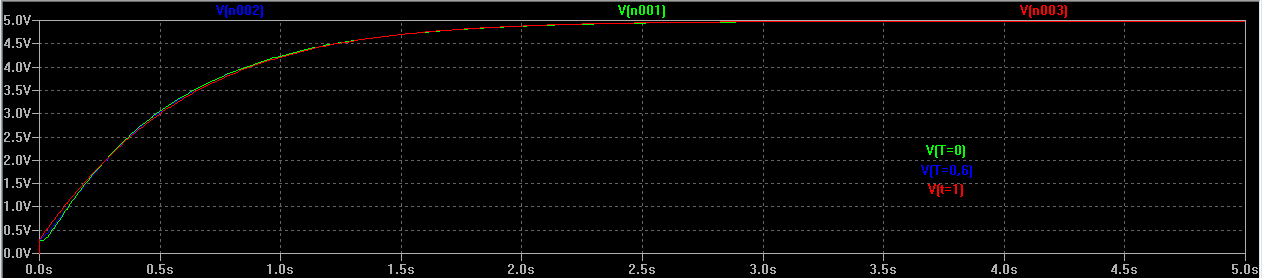
\includegraphics[width=3in]{img/simulacion47.png}
	\caption{Gráfica obtenidas al simular los circuitos con un condensador de 47 \(\mu F\) y con diferentes inductores en LTSpice}
	\label{fig:sim47}
\end{figure}
\begin{table}[]
	\centering
	\caption{Mediciones simuladas con un capacitor de 100 \(\mu F\)}
	\label{simulado100}
	\begin{tabular}{|l|l|l|l|l|l|}
		\hline
		medido          & error          & medido           & error          & medido          & error         \\ \hline
		\multicolumn{2}{|c|}{\(\tau\) 0} & \multicolumn{2}{c|}{\(\tau\) 0,6} & \multicolumn{2}{c|}{\(\tau\) 1} \\ \hline
		1,7             & 1,45           & 1,7              & 1,45           & 1,72             & 0,29          \\ \hline
		2,77            & 1,77           & 2,77             & 1,77           & 2,77            & 1,77          \\ \hline
		3,4             & 0,58           & 3,4              & 0,58           & 3,4             & 0,58          \\ \hline
		3,78            & 0,27           & 3,78             & 0,27           & 3,78            & 0,27          \\ \hline
		4,01            & 0,25           & 4,01             & 0,25           & 4,01            & 0,25          \\ \hline
		4,14            & 0,84           & 4,14             & 0,84           & 4,14            & 0,84          \\ \hline
		4,22            & 0,71           & 4,22             & 0,71           & 4,22            & 0,71          \\ \hline
		4,27            & 1,84           & 4,27             & 1,84           & 4,27            & 1,84          \\ \hline
		4,3             & 1,15           & 4,3              & 1,15           & 4,3             & 1,15          \\ \hline
		4,324            & 0,6           & 4,324             & 0,6           & 4,324            & 0,6          \\ \hline
	\end{tabular}
\end{table}
\begin{figure}
	\centering
	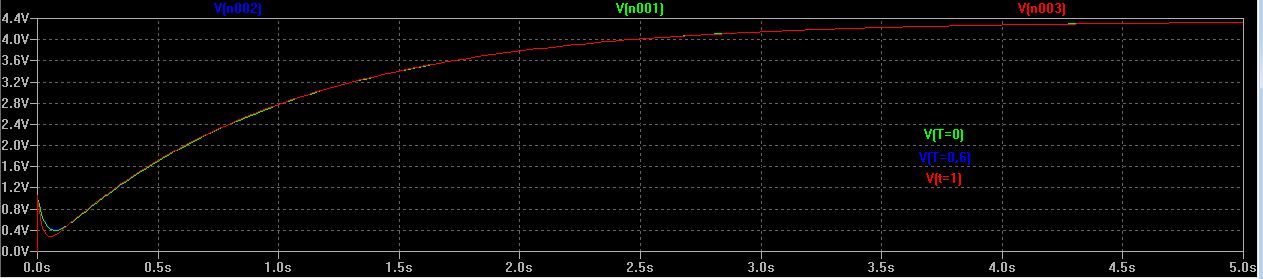
\includegraphics[width=3in]{img/simulacion100.png}
	\caption{Gráfica obtenidas al simular los circuitos con un condensador de 47 \(\mu F\) y  con diferentes inductores en LTSpice}
	\label{fig:sim100}
\end{figure}
\begin{table}[]
	\centering
	\caption{Mediciones simuladas con un capacitor de 10 \(\mu F\)}
	\label{simulado10}
	\begin{tabular}{|l|l|l|l|l|l|}
		\hline
		medido           & error          & medido           & error          & medido          & error         \\ \hline
		\multicolumn{2}{|c|}{\(\tau \) 0} & \multicolumn{2}{c|}{\(\tau\) 0,6} & \multicolumn{2}{c|}{\(\tau \)1} \\ \hline
		1,79             & 4,53           & 1,77             & 5,6            & 1,78            & 5,07          \\ \hline
		2,75             & 5,17           & 2,75             & 5,17           & 2,74            & 5,52          \\ \hline
		3,48             & 3,33           & 3,47             & 3,61           & 3,74            & 3,89          \\ \hline
		3,97             & 1,98           & 3,97             & 1,98           & 3,96            & 2,22          \\ \hline
		4,28             & 0,47           & 4,28             & 0,47           & 4,28            & 0,47          \\ \hline
		4,48             & 0,44           & 4,48             & 0,44           & 4,47            & 0,67          \\ \hline
		4,48             & 2,61           & 4,59             & 0,22           & 4,59            & 0,22          \\ \hline
		4,6              & 0,54           & 4,67             & 0,97           & 4,67            & 0,97          \\ \hline
		4,67             & 0,64           & 4,71             & 0,21           & 4,71            & 0,21          \\ \hline
		4,737            & 0,27           & 4,737            & 0,27           & 4,738           & 0,25          \\ \hline
	\end{tabular}
\end{table}
\begin{figure}
	\centering
	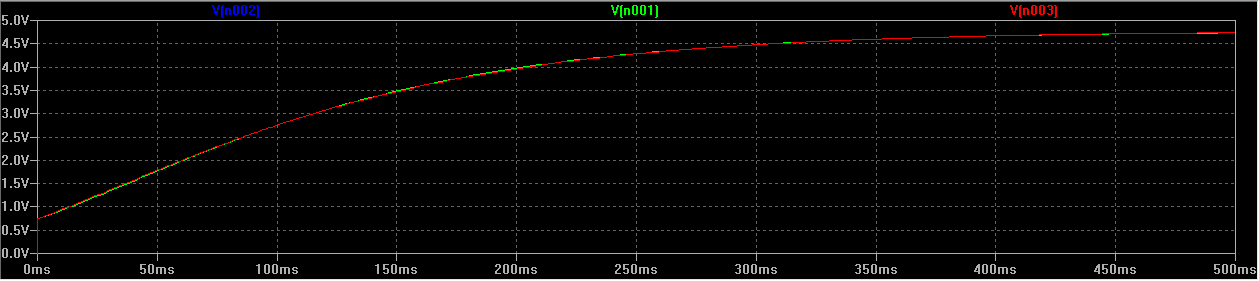
\includegraphics[width=3in]{img/simulacion10.png}
	\caption{Gráfica obtenidas al simular los circuitos con un condensador de 47 \(\mu F\) y  con diferentes inductores en LTSpice}
	\label{fig:sim10}
\end{figure}
% Reminder: the "draftcls" or "daftclsnofoot", not "draft", class option
% should be used if it is desired that the figures are to be displayed while
% in draft mode.

% An example of a floating figure using the graphicx package.
% Note that \label must occur AFTER (or within) \caption.
% For figures, \caption should occur after the \includegraphics.
%
%\begin{figure}
%\centering
%\includegraphics[width=2.5in]{myfigure}
% where an .eps filename suffix will be assumed under latex, 
% and a .pdf suffix will be assumed for pdflatex
%\caption{Simulation Results}
%\label{fig_sim}
%\end{figure}


% An example of a double column floating figure using two subfigures.
% (The subfigure.sty package must be loaded for this to work.)
% The subfigure \label commands are set within each subfigure command, the
% \label for the overall fgure must come after \caption.
% \hfil must be used as a separator to get equal spacing
%
%\begin{figure*}
%\centerline{\subfigure[Case I]{\includegraphics[width=2.5in]{subfigcase1}
% where an .eps filename suffix will be assumed under latex, 
% and a .pdf suffix will be assumed for pdflatex
%\label{fig_first_case}}
%\hfil
%\subfigure[Case II]{\includegraphics[width=2.5in]{subfigcase2}
% where an .eps filename suffix will be assumed under latex, 
% and a .pdf suffix will be assumed for pdflatex
%\label{fig_second_case}}}
%\caption{Simulation results}
%\label{fig_sim}
%\end{figure*}



% An example of a floating table. Note that, for IEEE style tables, the 
% \caption command should come BEFORE the table. Table text will default to
% \footnotesize as IEEE normally uses this smaller font for tables.
% The \label must come after \caption as always.
%
%\begin{table}
%% increase table row spacing, adjust to taste
%\renewcommand{\arraystretch}{1.3}
%\caption{An Example of a Table}
%\label{table_example}
%\centering
%% Some packages, such as MDW tools, offer better commands for making tables
%% than the plain LaTeX2e tabular which is used here.
%\begin{tabular}{|c||c|}
%\hline
%One & Two\\
%\hline
%Three & Four\\
%\hline
%\end{tabular}
%\end{table}


\section{Conclusiones}
\begin{itemize}
	\item El modelo propuesto reduce el error en el calculo de la carga del capacitor, en algunos casos hasta en un 9\%.
	\item El modelo con el que se trabajo funciona mejor en zonas de la carga lejanas al origen, ya que los cambios bruscos de la entrada alteran en gran medida a la salida.
	\item Los componentes que se usan en el modelo no representan los elementos físicos del condensador, sino como se puede representar mejor en la simulación.
	\item Para aproximar los valores de los inductores se debe tomar la década anterior al 0 en la gráfica del inductor como 0, puesto que la función de transferencia del inductor posee un polo en 0 este tendera a ser infinito.
\end{itemize}

% if have a single appendix:
%\appendix[Proof of the Zonklar Equations]
% or
%\appendix  % for no appendix heading
% do not use \section anymore after \appendix, only \section*
% is possibly needed

% use appendices with more than one appendix
% then use \section to start each appendix
% you must declare a \section before using any
% \subsection or using \label (\appendices by itself
% starts a section numbered zero.)
%
% Use this command to get the appendices' numbers in "A", "B" instead of the
% default capitalized Roman numerals ("I", "II", etc.).
% However, the capital letter form may result in awkward subsection numbers
% (such as "A-A"). Capitalized Roman numerals are the default.
%\useRomanappendicesfalse
%
\appendices
\section{gráficas de respuesta en frecuencias de los inductores}
Las figuras \ref{fig:bodeinductor47}, \ref{fig:bodeinductor100} y \ref{fig:bodeinductor10} representan el valor de las inductancias usando las formula \ref{eq:indutor_funcion} y graficadas en el programa WolframeAlpha con los valores de la tabla \ref{Table:Cparasitos}.
\begin{figure}
	\centering
	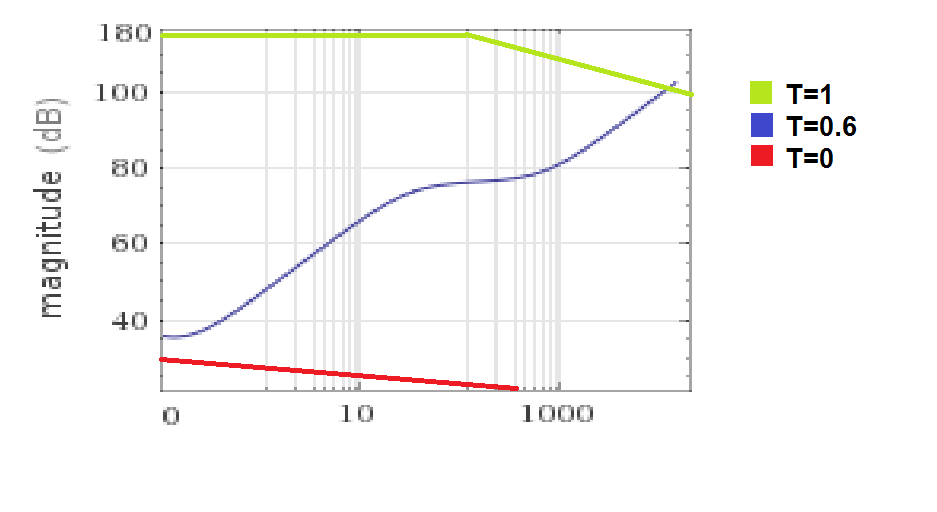
\includegraphics[width=2.5in]{img/bode47.png}
	\caption{Gráfica de bode de magnitud del capacitor de 47 \(\mu F\) con diferentes \(\tau\)}
	\label{fig:bodeinductor47}
\end{figure}
\begin{figure}
	\centering
	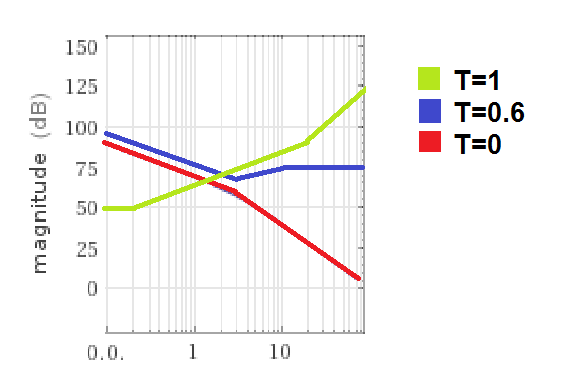
\includegraphics[width=2.5in]{img/bode100.png}
	\caption{Gráfica de bode de magnitud del capacitor de 100 \(\mu F\) con diferentes \(\tau\)}
	\label{fig:bodeinductor100}
\end{figure}
\begin{figure}
	\centering
	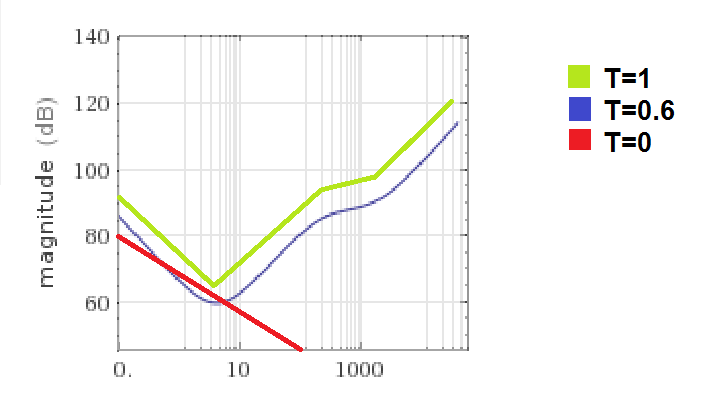
\includegraphics[width=2.5in]{img/bode10.png}
	\caption{Gráfica de bode de magnitud del capacitor de 10 \(\mu F\) con diferentes \(\tau\)}
	\label{fig:bodeinductor10}
\end{figure}

% you can choose not to have a title for an appendix
% if you want by leaving the argument blank


% trigger a \newpage just before the given reference
% number - used to balance the columns on the last page
% adjust value as needed - may need to be readjusted if
% the document is modified later
%\IEEEtriggeratref{8}
% The "triggered" command can be changed if desired:
%\IEEEtriggercmd{\enlargethispage{-5in}}

% references section
% NOTE: BibTeX documentation can be easily obtained at:
% http://www.ctan.org/tex-archive/biblio/bibtex/contrib/doc/

% can use a bibliography generated by BibTeX as a .bbl file
% standard IEEE bibliography style from:
% http://www.ctan.org/tex-archive/macros/latex/contrib/supported/IEEEtran/bibtex
%\bibliographystyle{IEEEtran.bst}
% argument is your BibTeX string definitions and bibliography database(s)
%\bibliography{IEEEabrv,../bib/paper}
%
% <OR> manually copy in the resultant .bbl file
% set second argument of \begin to the number of references
% (used to reserve space for the reference number labels box)
\begin{thebibliography}{1}

\bibitem{dorf}
J. A. Svobda y R. C. Dorf, Circuitos electricos, Mexico: AlfaOmega, 2011.
\bibitem{Hayt}
W. H. Hayt y J. A. Buck, Teoría Electromagnética, Mc Graw Hill, 1991. 
\bibitem{Saiku}
M. N. O. Saiku, de Elementos Del Electromagnetismo, Mexico, Oxford University Press, 2003, pp. 336-339.
\bibitem{modelos}
P. A. Moya, de Sistemas y señales fundamentos matemáticos, Costa Rica, Escuela ingeniería electrónica Tecnológico de Costa Rica, Centro de desarrollo de material bibliográfico(CDMB), 2003, pp. 177, 212.
\end{thebibliography}

% biography section
% 
% If you have an EPS/PDF photo (graphicx package needed) extra braces are
% needed around the contents of the optional argument to biography to prevent
% the LaTeX parser from getting confused when it sees the complicated
% \includegraphics command within an optional argument. (You could create
% your own custom macro containing the \includegraphics command to make things
% simpler here.)
%\begin{biography}[{\includegraphics[width=1in,height=1.25in,clip,keepaspectratio]{mshell}}]{Michael Shell}
% where an .eps filename suffix will be assumed under latex, and a .pdf suffix
% will be assumed for pdflatex; or if you just want to reserve a space for
% a photo:


% You can push biographies down or up by placing
% a \vfill before or after them. The appropriate
% use of \vfill depends on what kind of text is
% on the last page and whether or not the columns
% are being equalized.

%\vfill

% Can be used to pull up biographies so that the bottom of the last one
% is flush with the other column.
%\enlargethispage{-5in}

% that's all folks
\end{document}


